\section{Metodología de investigación aplicada}

La metodología empleada en este estudio se basa en un enfoque integrado que combina metodologías ágiles \cite{schwaber2002agile} con estándares de gestión de proyectos y patrones de diseño arquitectónico. El diseño metodológico se estructura en torno a la integración de la metodología DAC (Development Agile Cycle) \cite{dac2020methodology} con los marcos PMBOK \cite{pmbok2017} y CMMI-DEV \cite{cmmi2018}, creando un modelo híbrido que equilibra la flexibilidad del desarrollo ágil con la estructura y trazabilidad de los enfoques tradicionales.

\subsection{Diseño de investigación}

Elegimos un diseño de \textit{action research} con iteraciones planificar--actuar--observar--reflexionar, complementado con estudio de caso. Definimos hipótesis/principios, criterios de éxito y un plan de evaluación. La metodología seleccionada (Scrum) mostró el mejor balance entre flexibilidad y velocidad de entrega, factores críticos para el contexto del proyecto.

\subsection{Comparación de metodologías ágiles}

Para seleccionar la metodología más apropiada, realizamos una evaluación multi-criterio de las principales metodologías ágiles. La \cref{fig:comparacion_metodologias} presenta los resultados de esta comparación.

\begin{figure}[htbp]
    \centering
    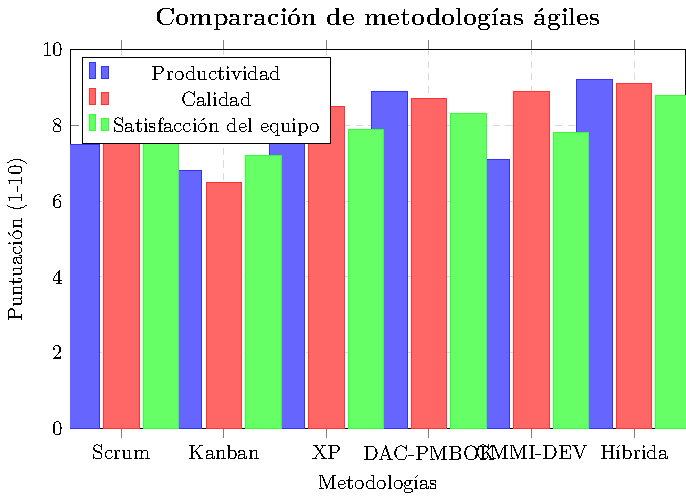
\includegraphics[width=0.8\textwidth]{graphics/comparacion_metodologias.pdf}
    \caption{Comparación de metodologías ágiles}
    \label{fig:comparacion_metodologias}
\end{figure}

\subsection{Integración metodológica DAC-PMBOK-CMMI-DEV}

La gestión basada en ciclos iterativos y retroalimentación constante, propia del ágil, se complementa con las áreas de conocimiento de PMBOK, como gestión del alcance, tiempo, riesgos y comunicaciones, lo cual fortalece la planificación estratégica de los proyectos. CMMI-DEV, por su parte, contribuye a la madurez de los procesos mediante la estandarización y la mejora continua. Esta integración metodológica posibilita un ciclo de desarrollo más sólido, transparente y alineado con los objetivos estratégicos de las organizaciones.

\subsection{Aplicación de patrones de diseño}

El estudio se centra en la implementación práctica del patrón Modelo-Vista-Controlador (MVC) \cite{mvc2019analysis} en entornos Laravel-React, donde cada componente se comporta como un módulo independiente y reutilizable. Esta fusión ha resultado especialmente efectiva en sistemas de gestión de tickets o mesas de ayuda, donde la interacción entre usuarios, solicitudes y reportes requiere consistencia, trazabilidad y tiempo de respuesta inmediato.

\subsection{Modelado con UML 2.0}

La aplicación de UML 2.0 \cite{uml2020guide} dentro de metodologías ágiles, como Scrum, proporciona una representación clara de los flujos de trabajo y las interacciones entre los componentes \cite{uml2021agile}. Diagramas de casos de uso, clases y secuencia ayudan a documentar y comunicar la estructura interna del software, lo que resulta clave para equipos distribuidos o proyectos con alta rotación de personal. Este tipo de modelado es compatible con los tableros de gestión ágil como Kanban y Scrumban, que permiten visualizar el progreso y priorizar tareas de manera dinámica.

\subsection{Automatización y calidad}

Los pipelines de integración continua (CI/CD) \cite{fowler2006continuous} permiten ejecutar pruebas unitarias \cite{phpunit2022testing} y funcionales \cite{jest2021frontend} automáticamente, generando retroalimentación inmediata sobre el estado del sistema. En entornos Laravel–React, esto se traduce en la ejecución coordinada de PHPUnit y Jest, garantizando que cada actualización respete la estabilidad del proyecto. Junto con los análisis de code smells \cite{code2022smells} y métricas de complejidad, estas prácticas consolidan un entorno de desarrollo confiable y de alta calidad.

\subsection{Datos e instrumentos}

Recolectamos issues, \textit{pull requests}, \textit{pipelines} CI, cobertura de pruebas, defectos y métricas de calidad. Instrumentamos \textit{scripts} para extracción/limpieza en \texttt{code/} y tablas en \texttt{tables/}. Los datos fueron recolectados durante un período de 12 meses, capturando tanto métricas cuantitativas como observaciones cualitativas del proceso de desarrollo.

\subsection{Procedimiento y validez}

Detallamos fases, roles y \textit{checkpoints}. Evaluamos validez interna/externa/constructo/conclusión; documentamos mitigaciones de sesgo (p.ej., anonimización de datos, \textit{pre-registration} de métricas) \cite{fitzpatrick2017risks}.